\documentclass{beamer}
\usepackage[latin1]{inputenc}
\usepackage{times}
\usepackage{tikz}
\usetheme{Luebeck}
%\usecolortheme{albatross}
\usepackage{amsmath,amsfonts,amsthm,amssymb}
\usepackage{setspace}
\usepackage{Tabbing}
\usepackage{fancyhdr}
\usepackage{lastpage}
\usepackage{extramarks}
\usepackage{chngpage}
\usepackage{soul,color}
\usepackage{graphicx,float,wrapfig}
\usepackage{xcolor}
\usepackage{listings}
\usepackage{float}
%\usepackage{subfloat}
\usepackage{subfigure}
\usepackage{caption}
\usepackage{enumitem}
\usepackage{algpseudocode}

\definecolor{darkorange}{RGB}{240, 120, 0}
\definecolor{darkgreen}{RGB}{0, 128, 0}
\definecolor{darkred}{RGB}{128, 0, 0}

\setbeamercolor{background canvas}{bg=white}
\setbeamercolor{frametitle}{fg=white, bg=darkorange}
\setbeamercolor{normal text}{bg=black,fg=black}
\setbeamercolor{structure}{bg=black, fg=darkorange}


\lstdefinestyle{customc}{
  belowcaptionskip=1\baselineskip,
  breaklines=true,
  frame=L,
  xleftmargin=\parindent,
  language=Python,
  showstringspaces=false,
  basicstyle=\footnotesize\ttfamily,
  keywordstyle=\bfseries\color{green!40!black},
  commentstyle=\itshape\color{purple!40!black},
  identifierstyle=\color{blue},
  stringstyle=\color{orange},
}

\lstdefinestyle{customc}{
  belowcaptionskip=1\baselineskip,
  breaklines=true,
  frame=L,
  xleftmargin=\parindent,
  language=Python,
  showstringspaces=false,
  basicstyle=\footnotesize\ttfamily,
  keywordstyle=\bfseries\color{green!40!black},
  commentstyle=\itshape\color{purple!40!black},
  identifierstyle=\color{blue},
  stringstyle=\color{orange},
}

\lstdefinestyle{customcsmall}{
  belowcaptionskip=1\baselineskip,
  breaklines=true,
  frame=L,
  xleftmargin=\parindent,
  language=Python,
  showstringspaces=false,
  basicstyle=\footnotesize\ttfamily,
  keywordstyle=\bfseries\color{green!24!black},
  commentstyle=\itshape\color{purple!24!black},
  identifierstyle=\color{blue},
  stringstyle=\color{orange},
}

\lstdefinestyle{customcsmall}{
  belowcaptionskip=1\baselineskip,
  breaklines=true,
  frame=L,
  xleftmargin=\parindent,
  language=Python,
  showstringspaces=false,
  basicstyle=\footnotesize\ttfamily,
  keywordstyle=\bfseries\color{green!24!black},
  commentstyle=\itshape\color{purple!24!black},
  identifierstyle=\color{blue},
  stringstyle=\color{orange},
}

\definecolor{MidGreen}{HTML}{00AA00}
\definecolor{MidYellow}{HTML}{AAAA00}

\title{Lecture 23: Spectral Meshes}
\date{4/7/2016}
\institute{Chris Tralie, Duke University}
\author{COMPSCI/MATH 290-04}
\begin{document}

\frame{\titlepage}

\begin{frame}{Announcements}
\begin{itemize}[label=$\vartriangleright$]

\item First project milestone Monday 4/11/2016

\item Final Project Rubric Up

\item Group Assignment 3 Out Tomorrow or Saturday...

\end{itemize}

\end{frame}

\begin{frame}{Table of Contents}

\begin{itemize}[label=$\blacktriangleright$]
	\item Laplacian Mesh Editing Finish
\end{itemize}

\begin{itemize}[label=$\vartriangleright$]
	\item Laplacian Eigenfunctions / Eigenvectors
\end{itemize}

\begin{itemize}[label=$\vartriangleright$]
	\item Spectral Mesh Compression / Shape DNA
\end{itemize}

\end{frame}


\begin{frame}{Laplacian Mesh Editing: Anchors}

\begin{minipage}{0.45\textwidth}{
\begin{figure}[t]
    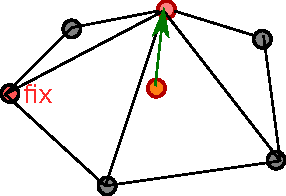
\includegraphics[width=0.7\textwidth]{2DDiscreteCurvatureAnchor1.pdf}
\end{figure}
}
\end{minipage}
\begin{minipage}{0.45\textwidth}
\[ \delta_i = \sum_{j \in N(i)} (v_i - v_j)\]

Delta coordinates define relative information about vertices with respect to their neighbors
\end{minipage}

\begin{figure}[t]
    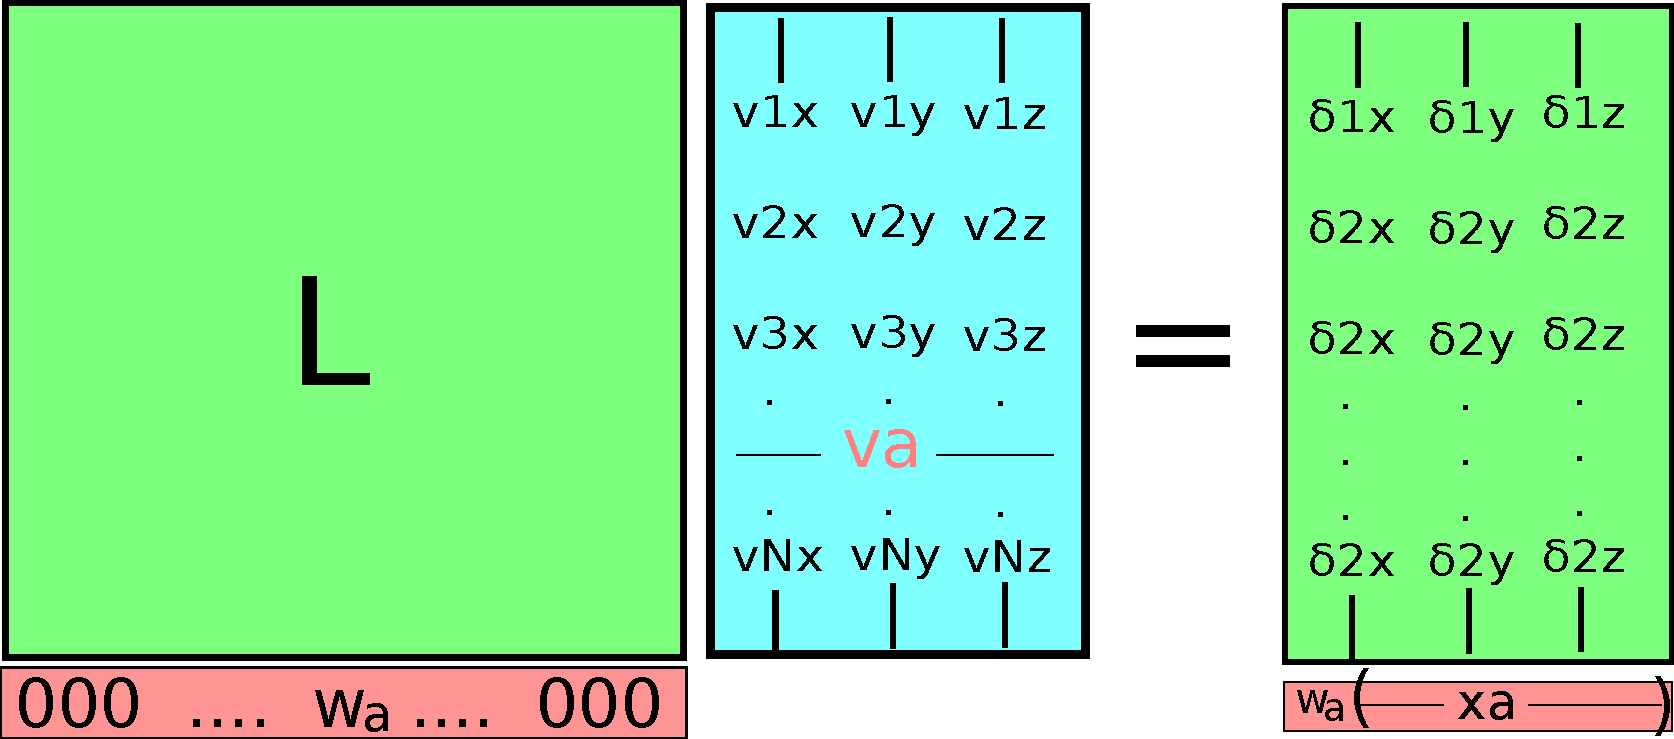
\includegraphics[width=0.8\textwidth]{LaplacianReconstruction1Anchor.pdf}
\end{figure}

\end{frame}


\begin{frame}{A Note About Rotation Invariance}

\[ \textcolor{darkgreen}{L} \textcolor{blue}{x} = \textcolor{darkgreen}{\delta} \]

\begin{itemize}[label=$\vartriangleright$]
\item $\delta$ is a {\em vector}.  $||\delta|| \propto \kappa$, but it has a direction
\end{itemize}

\begin{figure}[t]
    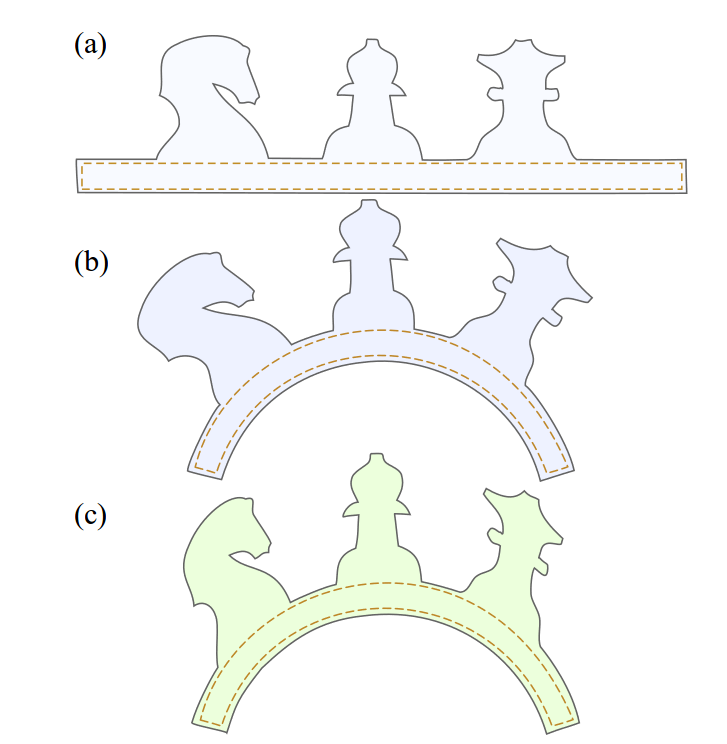
\includegraphics[width=0.5\textwidth]{Sorkine05.png}
    \caption{\textcolor{red}{Sorkine05}}
\end{figure}

\end{frame}

\begin{frame}{As Rigid As Possible Surface Editing}

\begin{figure}[t]
    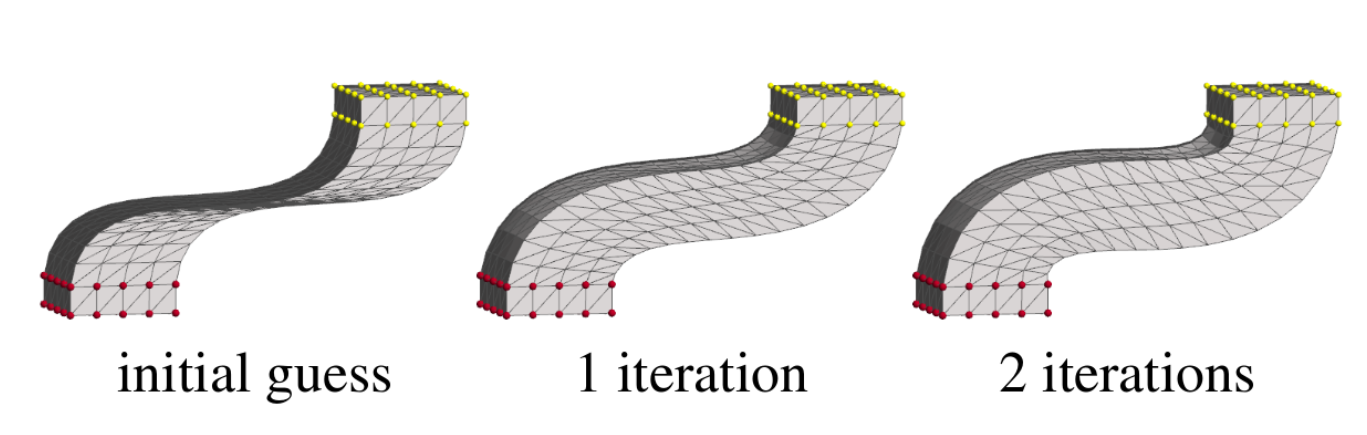
\includegraphics[width=\textwidth]{Sorkine07_1.png}
\end{figure}

\uncover<2->{
\begin{figure}[t]
    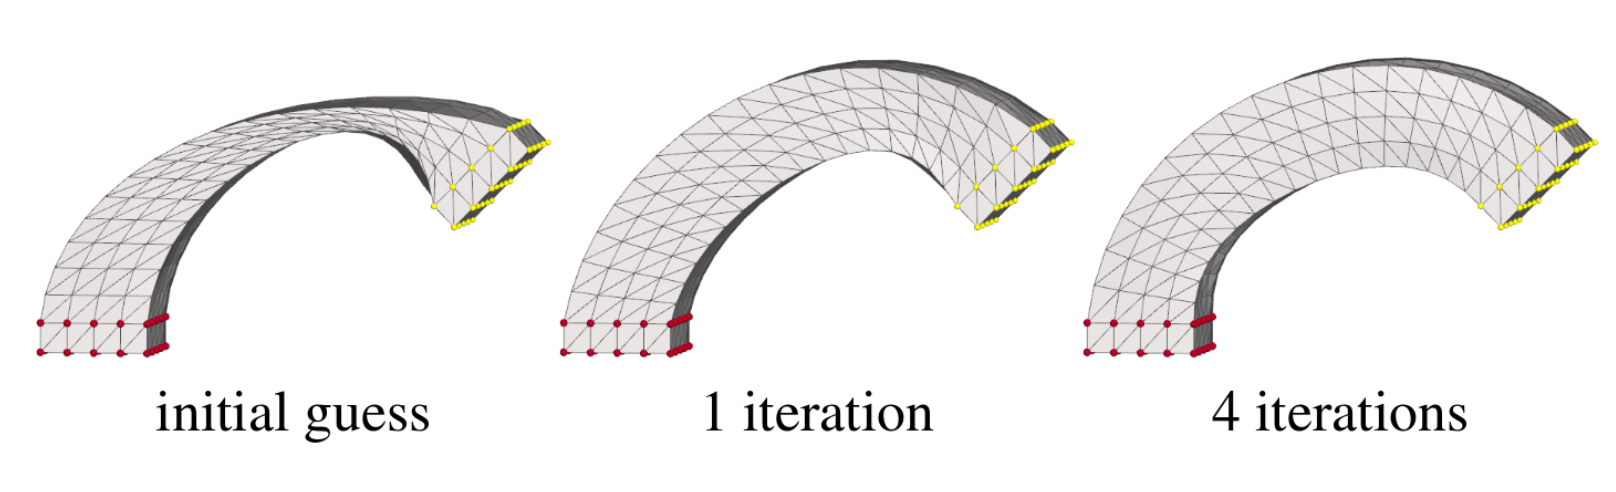
\includegraphics[width=\textwidth]{Sorkine07_2.png}
\end{figure}
}

\textcolor{red}{Sorkine2007}

\end{frame}



\begin{frame}{Table of Contents}

\begin{itemize}[label=$\vartriangleright$]
	\item Laplacian Mesh Editing Finish
\end{itemize}

\begin{itemize}[label=$\blacktriangleright$]
	\item Laplacian Eigenfunctions / Eigenvectors
\end{itemize}

\begin{itemize}[label=$\vartriangleright$]
	\item Spectral Mesh Compression / Shape DNA
\end{itemize}

\end{frame}

\begin{frame}{The 1D Second Derivative Operator}

Let $f(x) = \sin(\omega x)$

What is $f'(x)?$

\uncover<2->{
\[ f'(x) = \omega \cos(\omega x) \]
}

\uncover<3->{
What is $f''(x)$?
}

\uncover<4->{
\[ f''(x) = -\omega^2 \sin(\omega x) \]
}

\uncover<5->{
\[ f''(x) = -\omega^2 f(x) \]

We say sines and cosines are {\em eigenfunctions} of the second derivative operator and $-\omega^2$ is the associated {\em eigenvalue} (just like vectors!)
}

\end{frame}

\begin{frame}{1D Derivative Eigenfunctions}
Let $f(x) = \sin(\omega x)$, $f''(x) = -\omega^2 \sin(\omega x)$

\begin{figure}[t]
    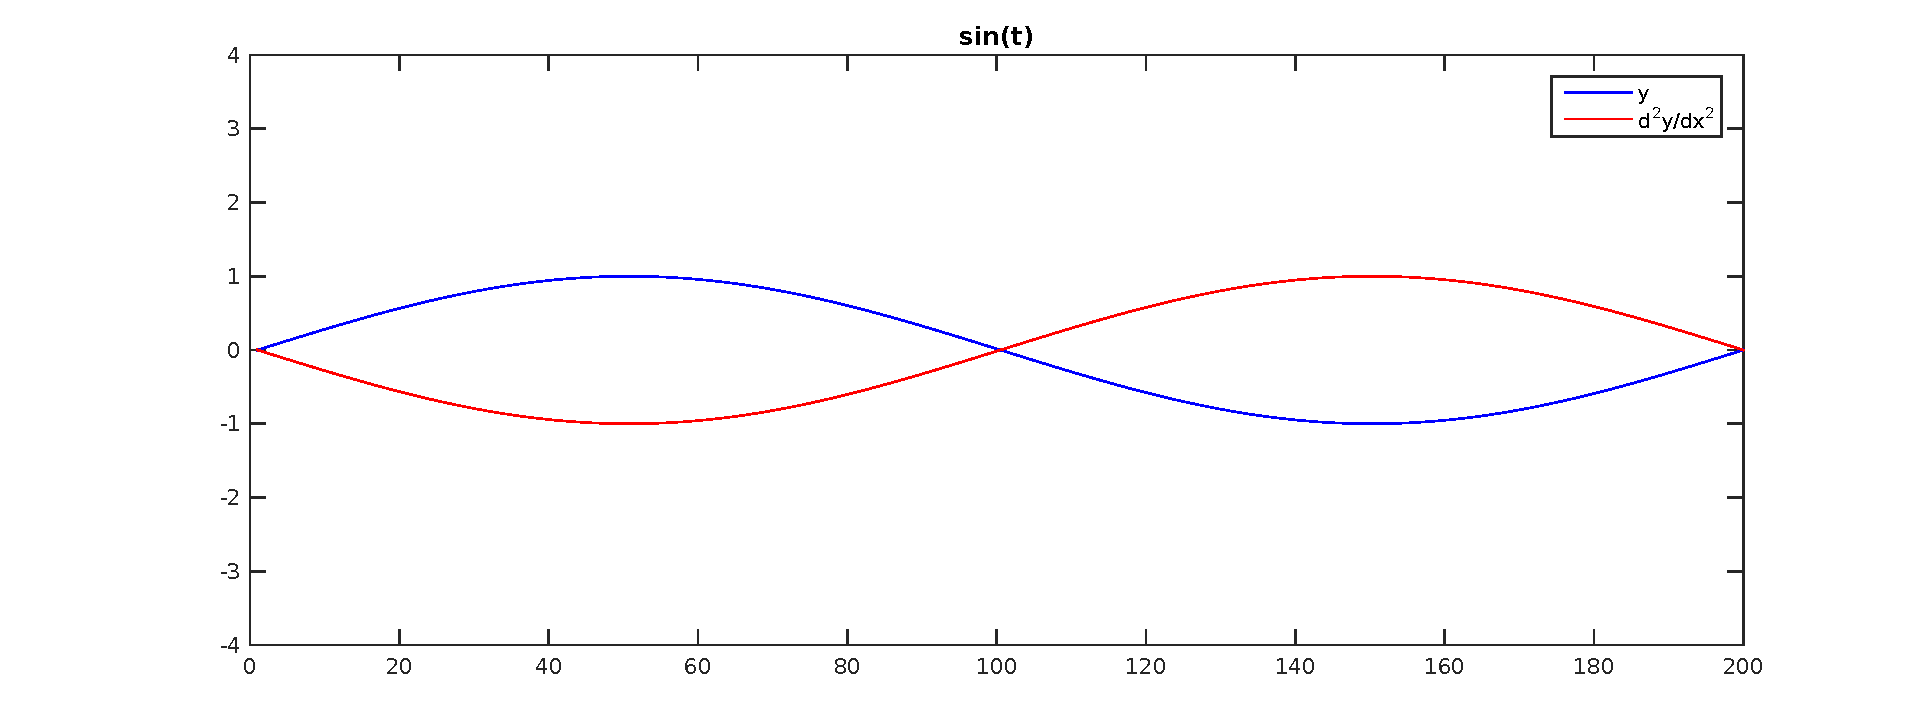
\includegraphics[width=0.7\textwidth]{cost.pdf}
\end{figure}

\begin{figure}[t]
    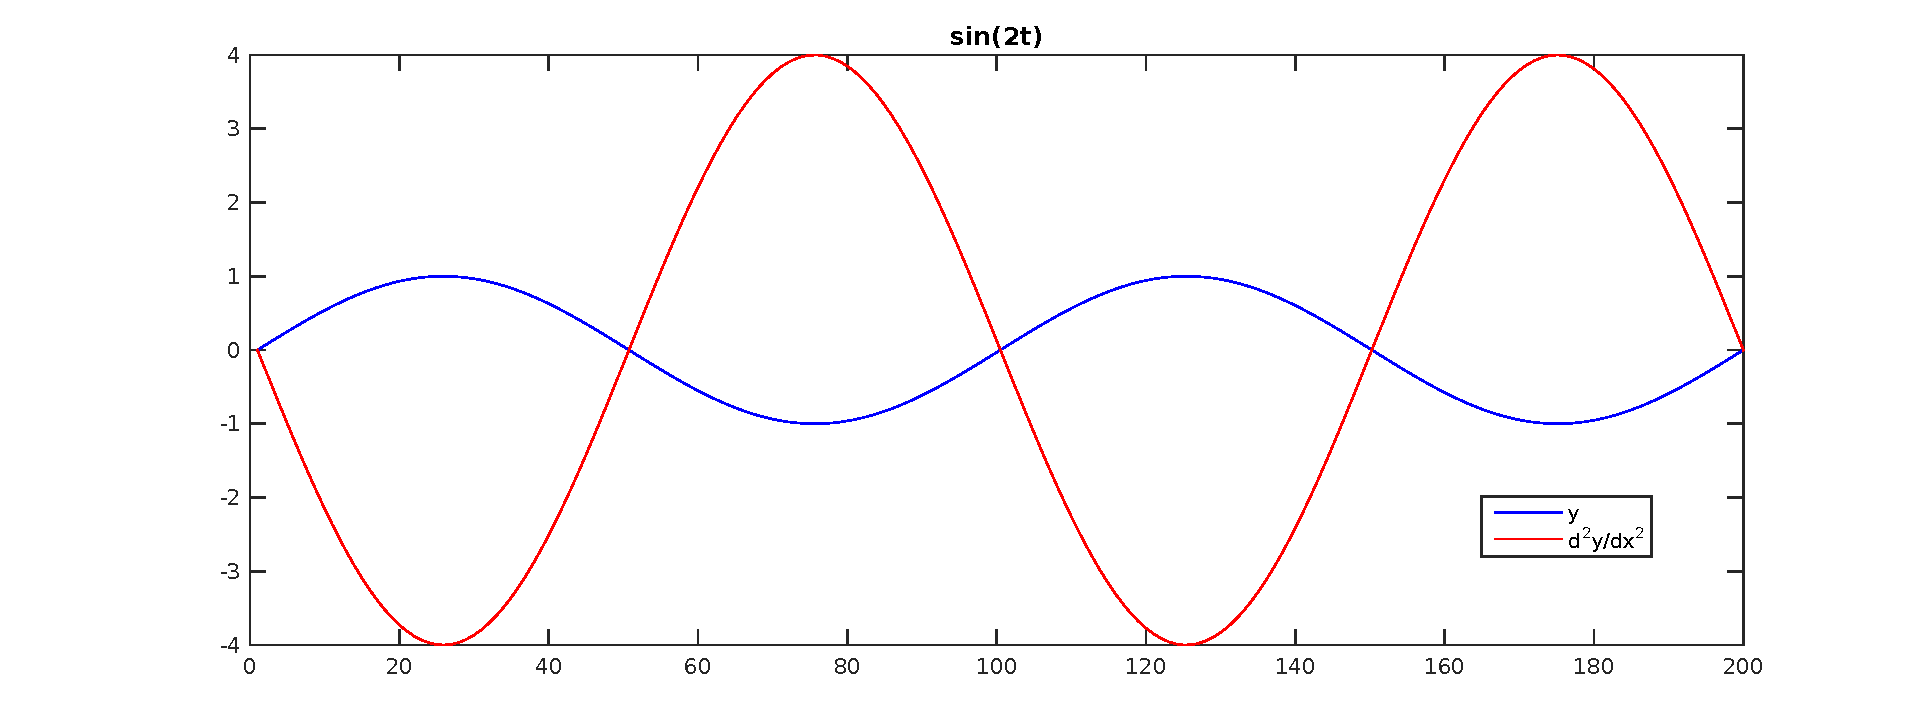
\includegraphics[width=0.7\textwidth]{cos2ts.pdf}
\end{figure}

Eigenvalues tell us frequency information

\end{frame}

\begin{frame}{Discrete Circle Laplacian}

\begin{figure}[t]
    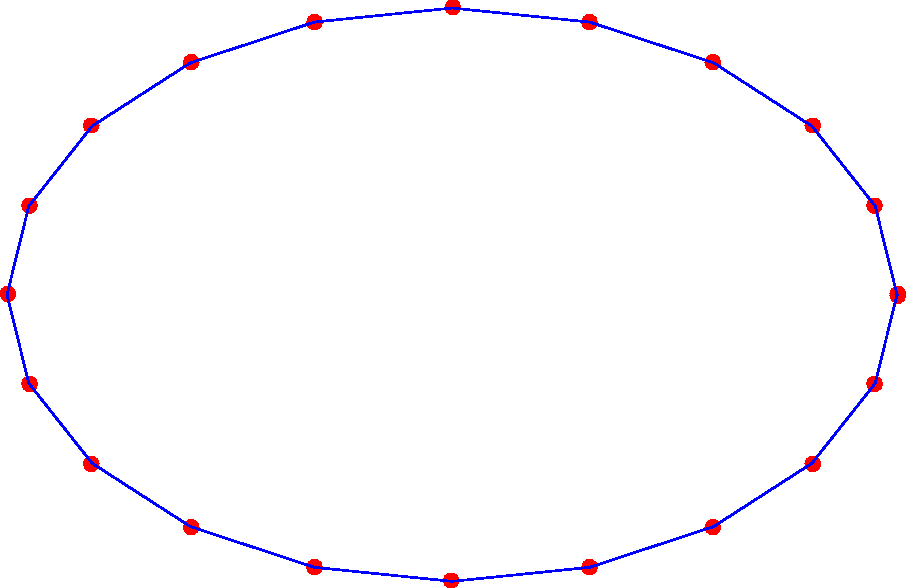
\includegraphics[width=0.32\textwidth]{CircleGraph.pdf}
\end{figure}

\begin{columns}
\uncover<2->{
\begin{column}[T]{5cm}
\begin{figure}[t]
    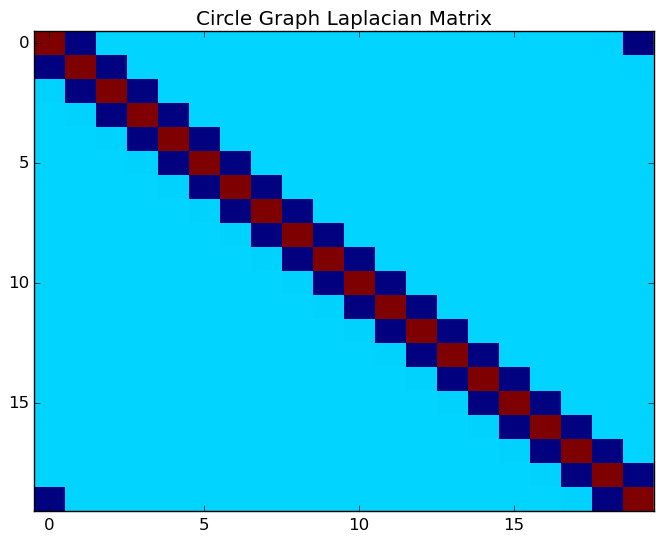
\includegraphics[width=\textwidth]{CircleLaplacian.png}
\end{figure}
\end{column}
}
\uncover<3->{
\begin{column}[T]{5cm}
\begin{figure}[t]
    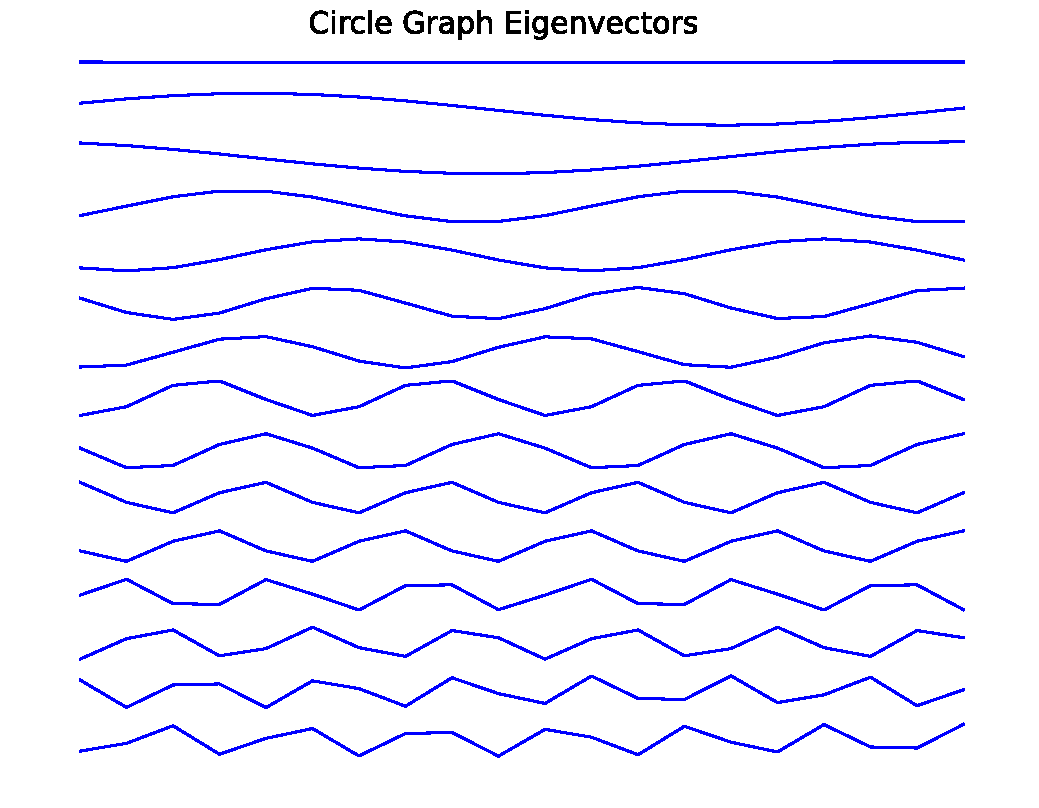
\includegraphics[width=\textwidth]{CircleEigvecs.pdf}
\end{figure}
\end{column}
}
\end{columns}

\tiny \url{https://github.com/COMPSCI290-S2016/NumpyDemos/blob/master/1DLaplacian.py}
\end{frame}


\begin{frame}{Laplacian of All 1s}

\[ L = D - A \]

\[ L \left[ \begin{array}{c} 1 \\ 1 \\ 1 \\ \vdots \\ 1 \end{array} \right] = ? \]

\end{frame}


\begin{frame}{Rect Eigenvectors}

\begin{columns}
\begin{column}[T]{5cm}
1
\begin{figure}[t]
    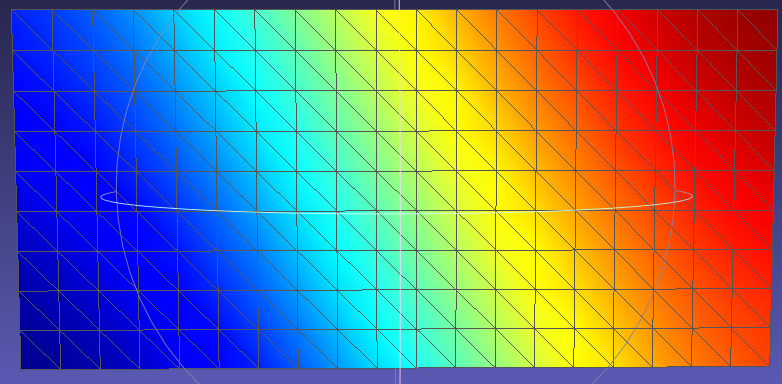
\includegraphics[width=\textwidth]{Harmonics/RectModes/rect1.png}
    %\caption*{\huge 0}
\end{figure}
2
\begin{figure}[t]
    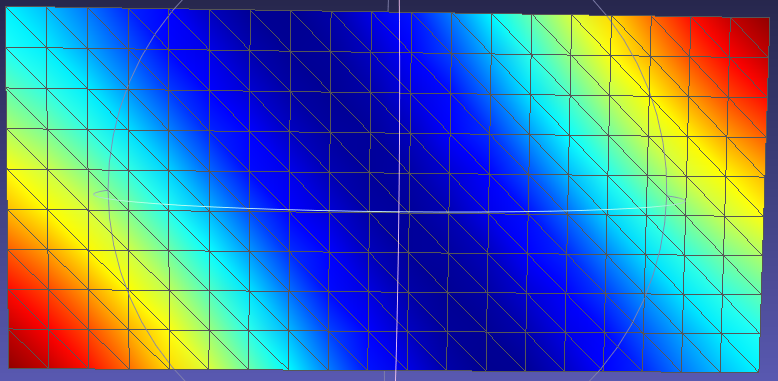
\includegraphics[width=\textwidth]{Harmonics/RectModes/rect2.png}
    %\caption*{\huge 1}
\end{figure}
\end{column}
\begin{column}[T]{5cm}
7
\begin{figure}[t]
    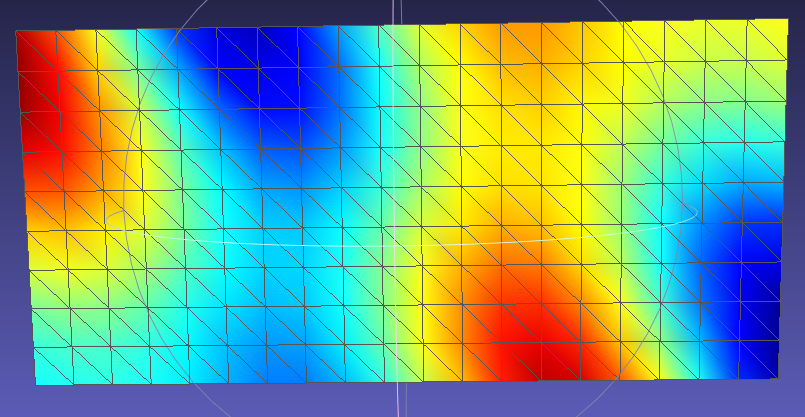
\includegraphics[width=\textwidth]{Harmonics/RectModes/rect7.png}
    %\caption*{\huge 0}
\end{figure}
8
\begin{figure}[t]
    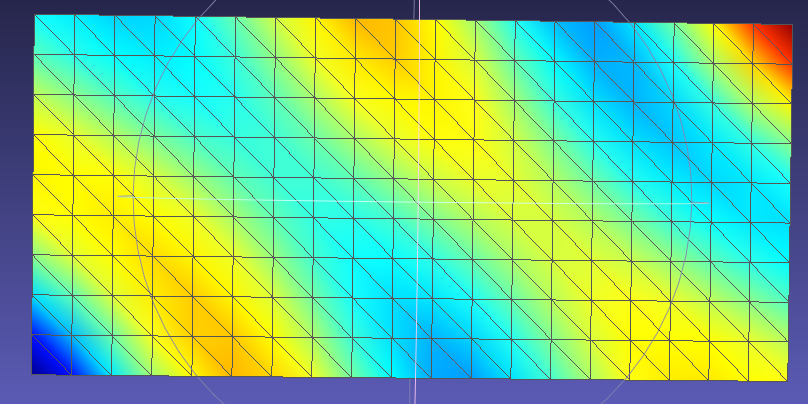
\includegraphics[width=\textwidth]{Harmonics/RectModes/rect8.png}
    %\caption*{\huge 1}
\end{figure}
\end{column}
\end{columns}

\end{frame}


\begin{frame}{Sphere Eigenvectors}

\uncover<2->{
\begin{columns}
\begin{column}[T]{5cm}
1
\begin{figure}[t]
    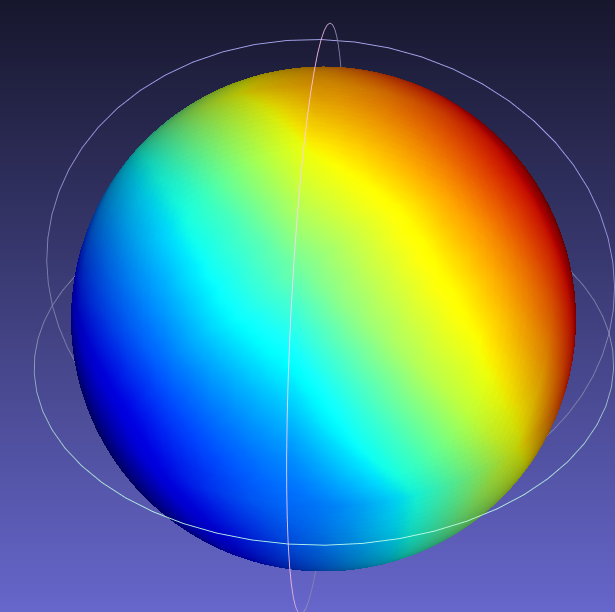
\includegraphics[width=0.6\textwidth]{Harmonics/SphereModes/sphere1.png}
    %\caption*{\huge 0}
\end{figure}
2
\begin{figure}[t]
    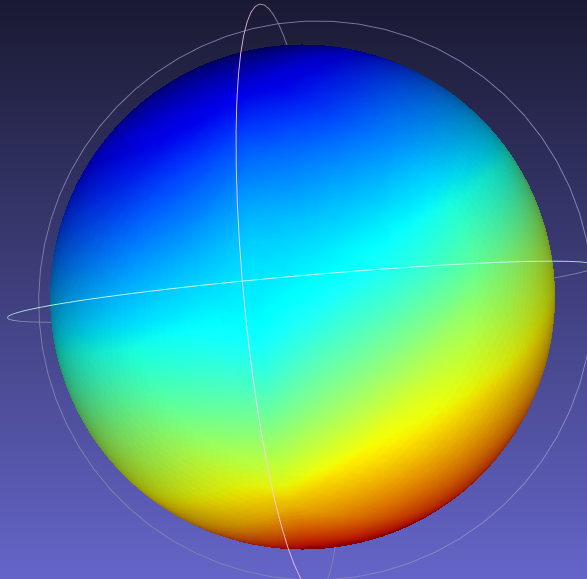
\includegraphics[width=0.6\textwidth]{Harmonics/SphereModes/sphere2.png}
    %\caption*{\huge 1}
\end{figure}
\end{column}
\begin{column}[T]{5cm}
7
\begin{figure}[t]
    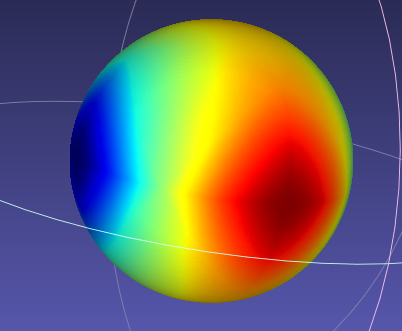
\includegraphics[width=0.6\textwidth]{Harmonics/SphereModes/sphere5.png}
    %\caption*{\huge 0}
\end{figure}
8
\begin{figure}[t]
    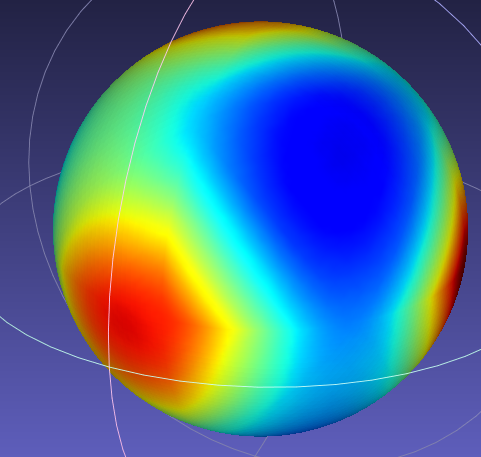
\includegraphics[width=0.6\textwidth]{Harmonics/SphereModes/sphere9.png}
    %\caption*{\huge 1}
\end{figure}
\end{column}
\end{columns}
}

\end{frame}


\begin{frame}{Homer Modes}

\begin{columns}
\begin{column}[T]{3cm}
\begin{figure}[t]
    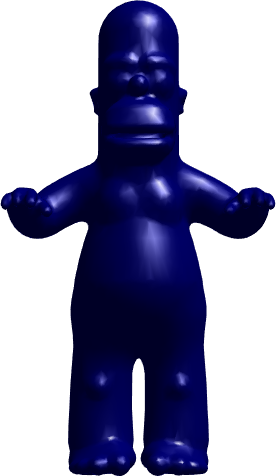
\includegraphics[width=\textwidth]{Harmonics/HomerModes/0.png}
    \caption*{\huge 0}
\end{figure}
\end{column}
\begin{column}[T]{3cm}
\begin{figure}[t]
    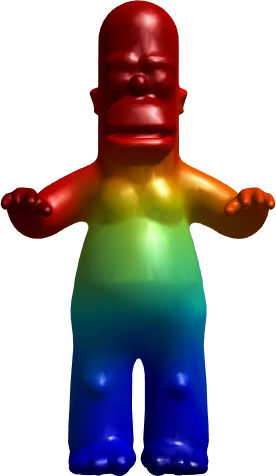
\includegraphics[width=\textwidth]{Harmonics/HomerModes/1.png}
    \caption*{\huge 1}
\end{figure}
\end{column}
\begin{column}[T]{3cm}
\begin{figure}[t]
    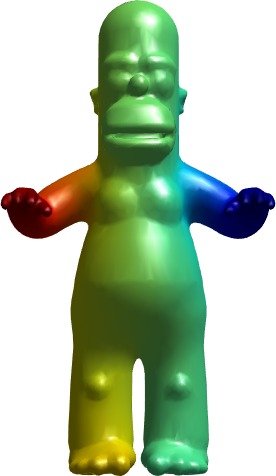
\includegraphics[width=\textwidth]{Harmonics/HomerModes/2.png}
    \caption*{\huge 2}
\end{figure}
\end{column}
\end{columns}

\end{frame}


\begin{frame}{Homer Modes}

\begin{columns}
\begin{column}[T]{3cm}
\begin{figure}[t]
    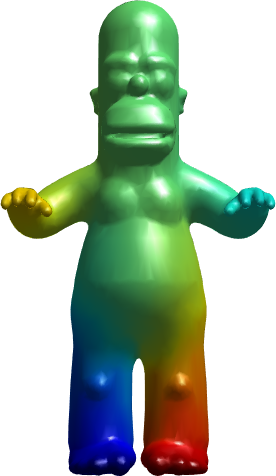
\includegraphics[width=\textwidth]{Harmonics/HomerModes/3.png}
    \caption*{\huge 3}
\end{figure}
\end{column}
\begin{column}[T]{3cm}
\begin{figure}[t]

    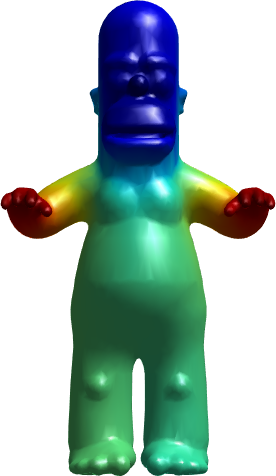
\includegraphics[width=\textwidth]{Harmonics/HomerModes/4.png}
    \caption*{\huge 4}
\end{figure}
\end{column}
\begin{column}[T]{3cm}
\begin{figure}[t]

    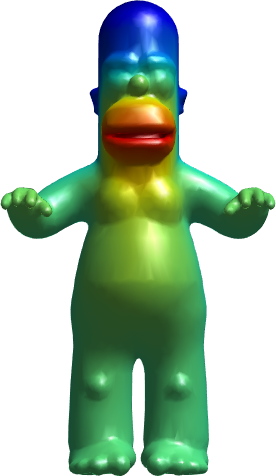
\includegraphics[width=\textwidth]{Harmonics/HomerModes/5.png}
    \caption*{\huge 5}
\end{figure}
\end{column}
\end{columns}

\end{frame}




\begin{frame}{Homer Modes}

\begin{columns}
\begin{column}[T]{3cm}
\begin{figure}[t]
    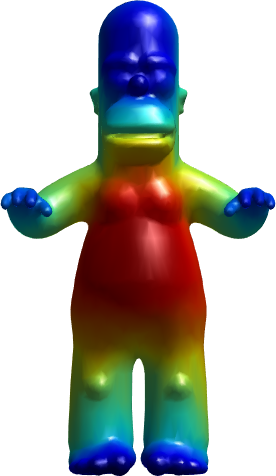
\includegraphics[width=\textwidth]{Harmonics/HomerModes/6.png}
    \caption*{\huge 6}
\end{figure}
\end{column}
\begin{column}[T]{3cm}
\begin{figure}[t]

    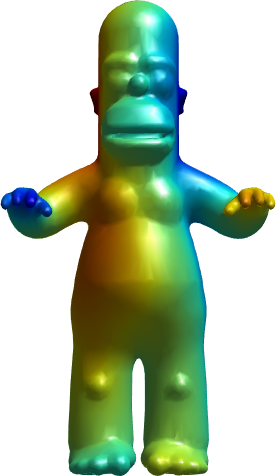
\includegraphics[width=\textwidth]{Harmonics/HomerModes/7.png}
    \caption*{\huge 7}
\end{figure}
\end{column}
\begin{column}[T]{3cm}
\begin{figure}[t]

    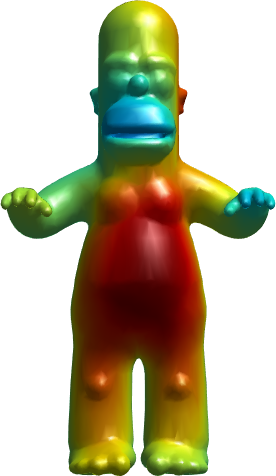
\includegraphics[width=\textwidth]{Harmonics/HomerModes/8.png}
    \caption*{\huge 8}
\end{figure}
\end{column}
\end{columns}

\end{frame}


\begin{frame}{Homer Modes}

\begin{columns}
\begin{column}[T]{3cm}
\begin{figure}[t]
    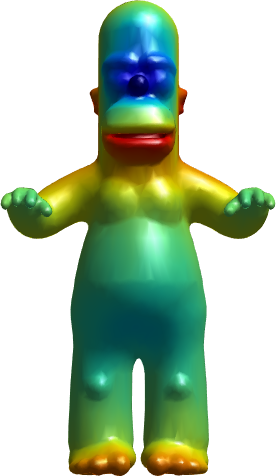
\includegraphics[width=\textwidth]{Harmonics/HomerModes/9.png}
    \caption*{\huge 9}
\end{figure}
\end{column}
\begin{column}[T]{3cm}
\begin{figure}[t]

    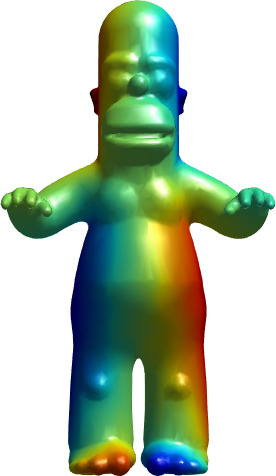
\includegraphics[width=\textwidth]{Harmonics/HomerModes/10.png}
    \caption*{\huge 10}
\end{figure}
\end{column}
\begin{column}[T]{3cm}
\begin{figure}[t]

    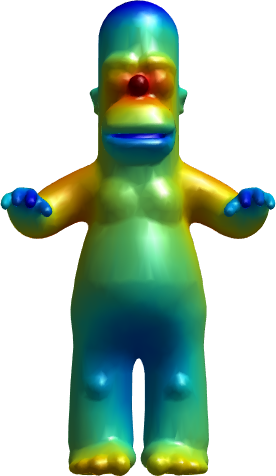
\includegraphics[width=\textwidth]{Harmonics/HomerModes/11.png}
    \caption*{\huge 11}
\end{figure}
\end{column}
\end{columns}

\end{frame}


\begin{frame}{Homer Modes}

\begin{columns}
\begin{column}[T]{3cm}
\begin{figure}[t]
    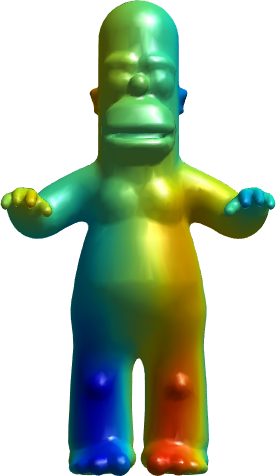
\includegraphics[width=\textwidth]{Harmonics/HomerModes/12.png}
    \caption*{\huge 12}
\end{figure}
\end{column}
\begin{column}[T]{3cm}
\begin{figure}[t]

    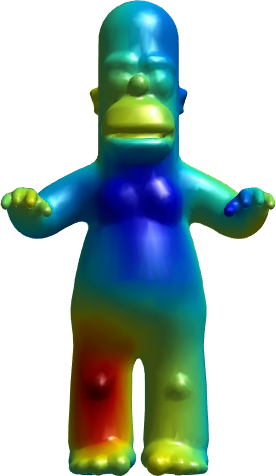
\includegraphics[width=\textwidth]{Harmonics/HomerModes/13.png}
    \caption*{\huge 13}
\end{figure}
\end{column}
\begin{column}[T]{3cm}
\begin{figure}[t]

    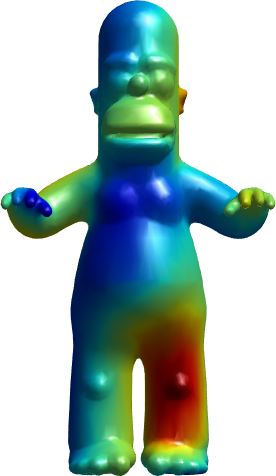
\includegraphics[width=\textwidth]{Harmonics/HomerModes/14.png}
    \caption*{\huge 14}
\end{figure}
\end{column}
\end{columns}

\end{frame}

\begin{frame}{Homer Modes}

\begin{columns}
\begin{column}[T]{3cm}
\begin{figure}[t]
    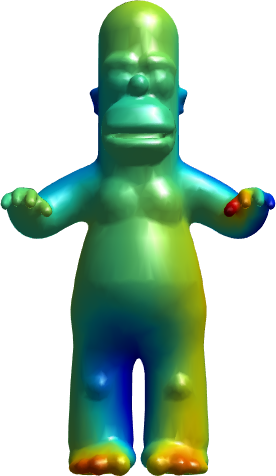
\includegraphics[width=\textwidth]{Harmonics/HomerModes/15.png}
    \caption*{\huge 15}
\end{figure}
\end{column}
\begin{column}[T]{3cm}
\begin{figure}[t]

    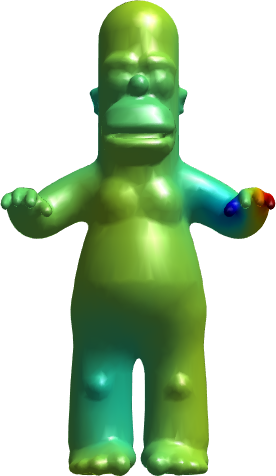
\includegraphics[width=\textwidth]{Harmonics/HomerModes/16.png}
    \caption*{\huge 16}
\end{figure}
\end{column}
\begin{column}[T]{3cm}
\begin{figure}[t]

    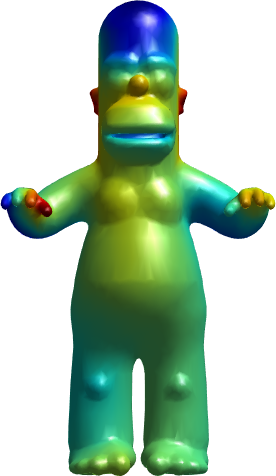
\includegraphics[width=\textwidth]{Harmonics/HomerModes/17.png}
    \caption*{\huge 17}
\end{figure}
\end{column}
\end{columns}

\end{frame}

\begin{frame}{Homer Modes}

\begin{columns}
\begin{column}[T]{3cm}
\begin{figure}[t]
    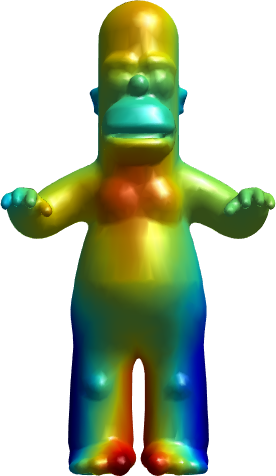
\includegraphics[width=\textwidth]{Harmonics/HomerModes/18.png}
    \caption*{\huge 18}
\end{figure}
\end{column}
\begin{column}[T]{3cm}
\begin{figure}[t]

    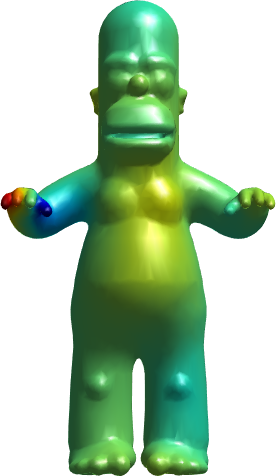
\includegraphics[width=\textwidth]{Harmonics/HomerModes/19.png}
    \caption*{\huge 19}
\end{figure}
\end{column}
\begin{column}[T]{3cm}
\begin{figure}[t]

    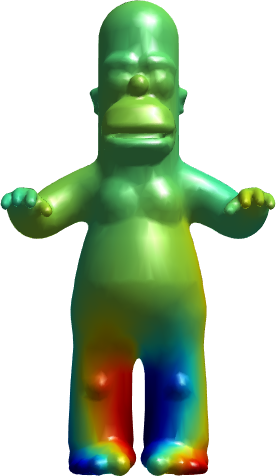
\includegraphics[width=\textwidth]{Harmonics/HomerModes/20.png}
    \caption*{\huge 20}
\end{figure}
\end{column}
\end{columns}

\end{frame}

\begin{frame}{Homer Modes}

\begin{figure}[t]
    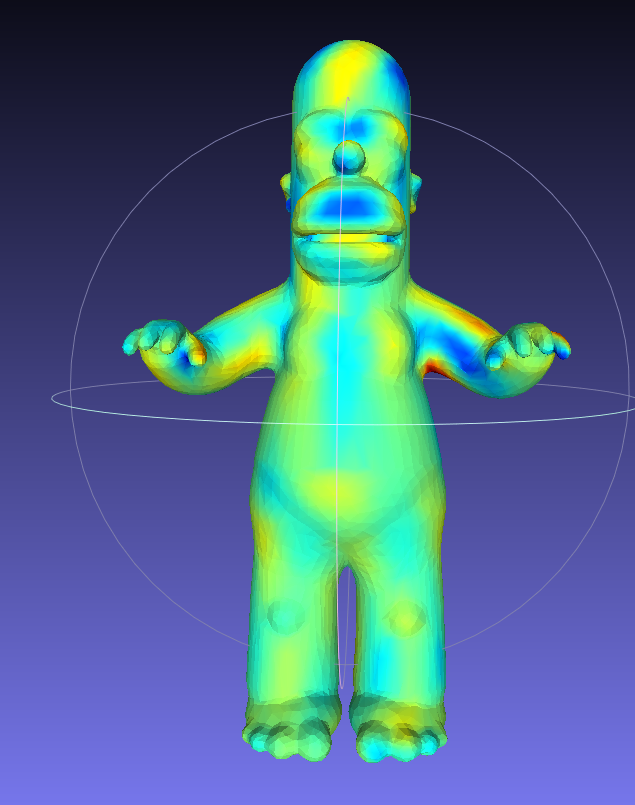
\includegraphics[width=0.5\textwidth]{homer200.png}
    \caption*{\huge 200}
\end{figure}

\end{frame}

\begin{frame}{Cheetah Modes}

\begin{columns}
\begin{column}[T]{5cm}
0
\begin{figure}[t]
    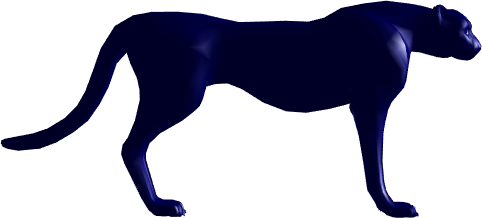
\includegraphics[width=\textwidth]{Harmonics/CheetahModes/0.png}
    %\caption*{\huge 0}
\end{figure}
2
\begin{figure}[t]
    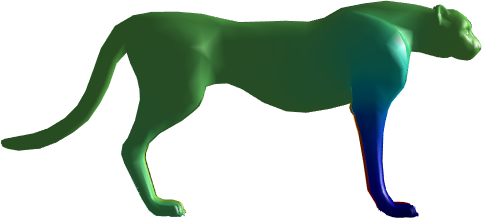
\includegraphics[width=\textwidth]{Harmonics/CheetahModes/2.png}
    %\caption*{\huge 1}
\end{figure}
\end{column}
\begin{column}[T]{5cm}
1
\begin{figure}[t]
    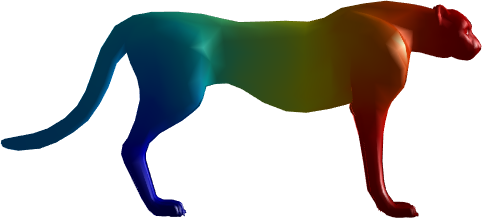
\includegraphics[width=\textwidth]{Harmonics/CheetahModes/1.png}
    %\caption*{\huge 0}
\end{figure}
3
\begin{figure}[t]
    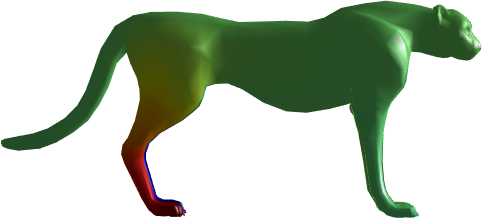
\includegraphics[width=\textwidth]{Harmonics/CheetahModes/3.png}
    %\caption*{\huge 1}
\end{figure}
\end{column}
\end{columns}

\end{frame}


\begin{frame}{Cheetah Modes}

\begin{columns}
\begin{column}[T]{5cm}
4
\begin{figure}[t]
    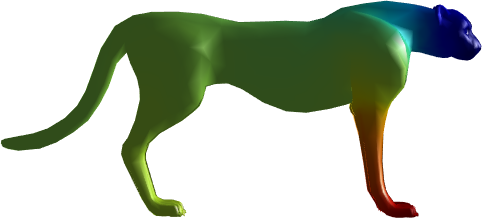
\includegraphics[width=\textwidth]{Harmonics/CheetahModes/4.png}
    %\caption*{\huge 0}
\end{figure}
6
\begin{figure}[t]
    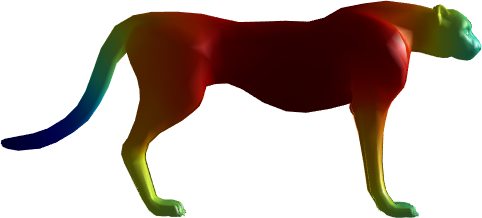
\includegraphics[width=\textwidth]{Harmonics/CheetahModes/6.png}
    %\caption*{\huge 1}
\end{figure}
\end{column}
\begin{column}[T]{5cm}
6
\begin{figure}[t]
    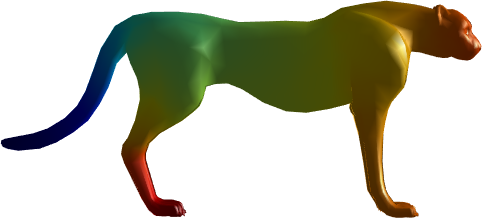
\includegraphics[width=\textwidth]{Harmonics/CheetahModes/5.png}
    %\caption*{\huge 0}
\end{figure}
7
\begin{figure}[t]
    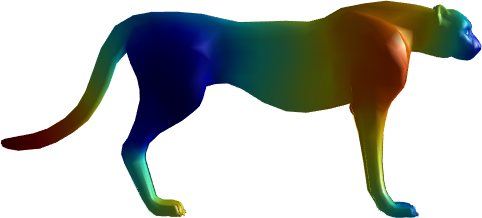
\includegraphics[width=\textwidth]{Harmonics/CheetahModes/7.png}
    %\caption*{\huge 1}
\end{figure}
\end{column}
\end{columns}

\end{frame}


\begin{frame}{Cheetah Modes}

\begin{columns}
\begin{column}[T]{5cm}
8
\begin{figure}[t]
    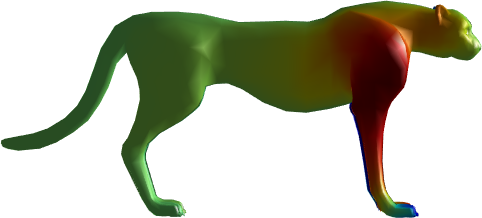
\includegraphics[width=\textwidth]{Harmonics/CheetahModes/8.png}
    %\caption*{\huge 0}
\end{figure}
10
\begin{figure}[t]
    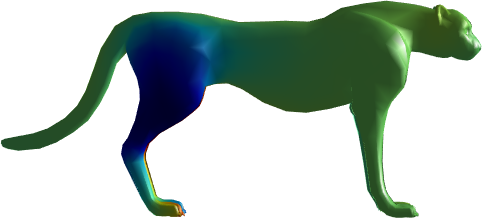
\includegraphics[width=\textwidth]{Harmonics/CheetahModes/10.png}
    %\caption*{\huge 1}
\end{figure}
\end{column}
\begin{column}[T]{5cm}
9
\begin{figure}[t]
    \includegraphics[width=\textwidth]{Harmonics/CheetahModes/9.png}
    %\caption*{\huge 0}
\end{figure}
11
\begin{figure}[t]
    \includegraphics[width=\textwidth]{Harmonics/CheetahModes/11.png}
    %\caption*{\huge 1}
\end{figure}
\end{column}
\end{columns}

\end{frame}


\begin{frame}{Cheetah Modes}

\begin{columns}
\begin{column}[T]{5cm}
12
\begin{figure}[t]
    \includegraphics[width=\textwidth]{Harmonics/CheetahModes/12.png}
    %\caption*{\huge 0}
\end{figure}
14
\begin{figure}[t]
    \includegraphics[width=\textwidth]{Harmonics/CheetahModes/14.png}
    %\caption*{\huge 1}
\end{figure}
\end{column}
\begin{column}[T]{5cm}
13
\begin{figure}[t]
    \includegraphics[width=\textwidth]{Harmonics/CheetahModes/13.png}
    %\caption*{\huge 0}
\end{figure}
15
\begin{figure}[t]
    \includegraphics[width=\textwidth]{Harmonics/CheetahModes/15.png}
    %\caption*{\huge 1}
\end{figure}
\end{column}
\end{columns}

\end{frame}


\begin{frame}{Cheetah Modes}

\begin{columns}
\begin{column}[T]{5cm}
16
\begin{figure}[t]
    \includegraphics[width=\textwidth]{Harmonics/CheetahModes/16.png}
    %\caption*{\huge 0}
\end{figure}
18
\begin{figure}[t]
    \includegraphics[width=\textwidth]{Harmonics/CheetahModes/18.png}
    %\caption*{\huge 1}
\end{figure}
\end{column}
\begin{column}[T]{5cm}
17
\begin{figure}[t]
    \includegraphics[width=\textwidth]{Harmonics/CheetahModes/17.png}
    %\caption*{\huge 0}
\end{figure}
19
\begin{figure}[t]
    \includegraphics[width=\textwidth]{Harmonics/CheetahModes/19.png}
    %\caption*{\huge 1}
\end{figure}
\end{column}
\end{columns}

\end{frame}


\begin{frame}{Cheetah Modes}

\begin{figure}[t]
    \includegraphics[width=\textwidth]{Cheetah399.png}
    \caption*{\huge 400}
\end{figure}

\end{frame}

\begin{frame}{Normalize Each Row By Degree?}
Why not $\hat{L} = D^{-1}A$?

\begin{figure}[t]
    \includegraphics[width=0.8\textwidth]{Sorkine05_GraphLaplacian.png}
\end{figure}
\small \textcolor{red}{Sorkine 05}

\uncover<2->{
 \[ \hat{L} \neq \hat{L^T} \text{    symmetry is broken..can't get real orthogonal eigenvectors}\]
}

\end{frame}


\begin{frame}{Table of Contents}

\begin{itemize}[label=$\vartriangleright$]
	\item Laplacian Mesh Editing Finish
\end{itemize}

\begin{itemize}[label=$\vartriangleright$]
	\item Laplacian Eigenfunctions / Eigenvectors
\end{itemize}

\begin{itemize}[label=$\blacktriangleright$]
	\item Spectral Mesh Compression / Shape DNA
\end{itemize}

\end{frame}


\begin{frame}{Recall: Sinusoidal Decomposition}
Project a function onto sinusoids, approximate with lower order sinusoids

\begin{columns}
\begin{column}[T]{5cm}
\begin{figure}[t]
    \includegraphics[width=\textwidth]{Sawtooth.png}
\end{figure}
\end{column}
\begin{column}[T]{5cm}
\begin{figure}[t]
    \includegraphics[width=\textwidth]{Gaussian.png}
\end{figure}
\end{column}
\end{columns}


This is ``lowpass filtering''
\end{frame}

\begin{frame}{Laplacian Eigenbasis Decomposition}
\[ L = D - A = USU^T \]

Let's project the coordinates of the mesh onto the truncated Laplacian eigen basis

\small
\[ \left[ \begin{array}{ccc} | & | & | \\ x' & y' & z' \\ | & | & | \end{array} \right] = \left[ \begin{array}{cccc} | & | & | & | \\ u_1 & u_2 & \hdots & u_K \\ | & | & | & | \end{array} \right] \left[ \begin{array}{ccc}  - & u_1 & - \\ - & u_2 & - \\ \vdots & \vdots & \vdots \\ - & u_K & - \end{array} \right] \left[ \begin{array}{ccc} | & | & | \\ x & y & z \\ | & | & |  \end{array} \right] \]

\[ X' = U_K U_K^T X \]

\end{frame}

\begin{frame}{Homer: 5000 Vertices}

10 Eigenvectors
\begin{figure}[t]
    \includegraphics[width=0.35\textwidth]{Harmonics/HomerProjections/Homer10.png}
\end{figure}

\end{frame}

\begin{frame}{Homer: 5000 Vertices}

20 Eigenvectors
\begin{figure}[t]
    \includegraphics[width=0.35\textwidth]{Harmonics/HomerProjections/Homer20.png}
\end{figure}

\end{frame}

\begin{frame}{Homer: 5000 Vertices}

50 Eigenvectors
\begin{figure}[t]
    \includegraphics[width=0.35\textwidth]{Harmonics/HomerProjections/Homer50.png}
\end{figure}

\end{frame}

\begin{frame}{Homer: 5000 Vertices}

100 Eigenvectors
\begin{figure}[t]
    \includegraphics[width=0.35\textwidth]{Harmonics/HomerProjections/Homer100.png}
\end{figure}

\end{frame}


\begin{frame}{Homer: 5000 Vertices}

500 Eigenvectors
\begin{figure}[t]
    \includegraphics[width=0.35\textwidth]{Harmonics/HomerProjections/Homer500.png}
\end{figure}

10x compression ratio for vertices!

\end{frame}


\begin{frame}{Cheetah: 2000 Vertices}

20 Eigenvectors
\begin{figure}[t]
    \includegraphics[width=\textwidth]{Harmonics/CheetahProjections/CheetahProj20.png}
\end{figure}

\end{frame}

\begin{frame}{Cheetah: 2000 Vertices}

100 Eigenvectors
\begin{figure}[t]
    \includegraphics[width=\textwidth]{Harmonics/CheetahProjections/CheetahProj100.png}
\end{figure}

\end{frame}


\begin{frame}{Cheetah: 2000 Vertices}

200 Eigenvectors
\begin{figure}[t]
    \includegraphics[width=\textwidth]{Harmonics/CheetahProjections/CheetahProj200.png}
\end{figure}

\end{frame}

\begin{frame}{Cheetah: 2000 Vertices}

400 Eigenvectors
\begin{figure}[t]
    \includegraphics[width=\textwidth]{Harmonics/CheetahProjections/CheetahProj400.png}
\end{figure}

\end{frame}

\begin{frame}{Can Also Use to Denoise}


\begin{columns}
\begin{column}[T]{5cm}
\begin{figure}[t]
    \includegraphics[width=0.8\textwidth]{NoisyHomer.png}
    \caption*{Noisy Homer}
\end{figure}
\end{column}
\begin{column}[T]{5cm}
\begin{figure}[t]
    \includegraphics[width=0.8\textwidth]{DenoisedHomer.png}
    \caption*{Projected Onto First 500 Eigenvectors}
\end{figure}
\end{column}
\end{columns}

\end{frame}

\begin{frame}{Compress Surface Patchwise}

\begin{figure}[t]
    \includegraphics[width=0.8\textwidth]{Karni2000.png}
\end{figure}

\small
\textcolor{red}{Karni 2000}

\begin{itemize}[label=$\vartriangleright$]
\item Avoids numerical stability issues, better picking up on local geometry

\item Like DCT for JPEG
\end{itemize}

\end{frame}

\begin{frame}{Shape DNA}
Histogram of eigenvalues, sorted in ascending order

\begin{figure}[t]
    \includegraphics[width=0.6\textwidth]{ShapeDNA.pdf}
\end{figure}

\begin{itemize}[label=$\vartriangleright$]
\item Invariant to {\em isometries}
\item Our first nonrigid shape descriptor!
\end{itemize}
\end{frame}

\end{document}

